\chapter{Implementierung}

In diesem Kapitel wird die Implementierung des Backends, Frontends und
Dashboards des Systems beschrieben. Die Implementierung basiert auf der in
\autoref{chapter:conception} erarbeiteten Konzeption. Zunächst wird der
generelle Aufbau des Projekts beschrieben. Anschließend wird das Backend
umgesetzt, welches sämtliche Daten des Systems speichert und die Speicherung und
Manipulation dieser durch entsprechende Schnittstellen ermöglicht. Hiernach wird
das Frontend entsprechend nach dem konzipierten Prototypen (s.
\autoref{sec:interface-design}) realisiert. Abschließend wird das Dashboard
implementiert.

\section{Struktur des Systems}



% Speichern von Nutzerdaten ohne konkrete Anmeldung

% Usability von interaktiven Karten
% - Alter
% - Behinderung
% - Technikaffinität

% Usability QR-Code Reader


\section{Implementierung des Backends}

In diesem Abschnitt werden die Struktur des Backends und Implementierung der
Funktionalitäten näher erläutert. Die zu implementierenden Funktionalitäten sind
aus \autoref{sec:concept-func} zu entnehmen. Anschließend werden Maßnahmen zur Sicherstellung der Softwarequalität beschrieben.

\subsection{Struktur eines Strapi-Projekts}

Im Folgenden wird die Struktur des Backends und seiner verschiedenen
Teilkomponenten erläutert. Die Verzeichnisstruktur wird in
\autoref{fig:impl-backend-structure} aufgezeigt. Zur bessern Lesbarkeit werden
einige Dateien und Unterverzeichnisse ausgeblendet. Das Strapi Projekt teilt
sich vier wesentliche Teilbereiche auf: API, Komponenten, Konfiguration und
Plugins. Diese vier Teilbereiche finden sich in der Verzeichnisstruktur in den
entsprechenden Ordnern wieder.

\begin{figure}[htpb]
    \centering
    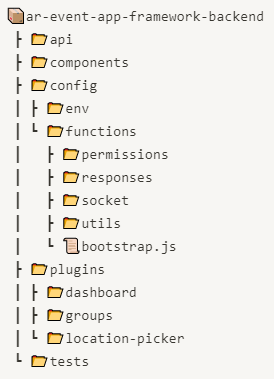
\includegraphics[width=.45\linewidth]{impl/dir_tree_backend.png}
    \caption{Verzeichnisstruktur des Backends}
    \label{fig:impl-backend-structure}
\end{figure}

Der \lstinline[style=code, style=inline]{/api} Ordner beinhaltet die
verschiedenen angelegten APIs des Strapi Projekts. Die meisten der APIs nutzen
hierbei Inhaltstypen (Content-Types). Inhaltstypen werden in Strapi genutzt, um
die Struktur und Art eines Inhalts zu definieren. Die Datenstruktur eines
Inhaltstyps wird dabei durch Attribute festgelegt, welche aus Name, Art und
einstellbaren Einschränkungen bestehen. Strapi stellt drei Arten von
Inhaltstypen bereit: Kollektionen, Einzeltypen und Komponenten. Während
Kollektionen eine Vielzahl von Einträgen beinhalten kann, bestehen Einzeltypen
aus nur einem Eintrag. Komponenten sind hingegen ein wiederverwendbarer
Inhaltstyp, welcher nur in Verbindung mit Kollektionen oder Einzeltypen genutzt
werden kann. Sie sind im \lstinline[style=code, style=inline]{/components}
Verzeichnis wiederzufinden. Die APIs des Systems sind in
\autoref{fig:impl-backend-apis} zu sehen.

\begin{figure}[htpb]
    \centering
    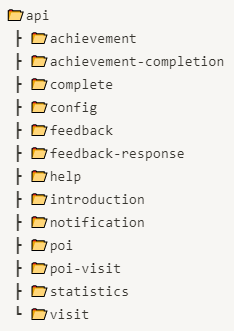
\includegraphics[width=.4\linewidth]{impl/dir_apis.png}
    \caption{Verzeichnisstruktur der Inhaltstypen}
    \label{fig:impl-backend-apis}
\end{figure}

Jede API wird wie folgt unterteilt (s. \autoref{fig:impl-backend-content-type}
zur Verzeichnisstruktur) und anschließend näher erläutert:

\begin{enumerate}
    \setlength{\itemsep}{1em}
    \item \textbf{Konfiguration (/config)} \\
          Zuweisung von Routen zu Kontroller-Funktionen unter Angabe von
          \textit{HTTP-Methode, URL} und \textit{Kontroller-Funktion}.
    \item \textbf{Kontroller (/controllers)} \\
          Enthält Funktionen, welche Anfragen, wie in der Konfiguration
          festgelegt, empfangen, verarbeiten und eine Antwort oder einen Fehler
          zurücksenden.
    \item \textbf{Modelle (/models)} \\
          Legt Datenstruktur und Name des Inhaltstypen fest. Die verfügbaren
          Datentypen werden in \autoref{fig:impl-backend-types} aufgelistet.
          Falls die API keinen Inhaltstypen nutzt, wird dieses Verzeichnis nicht
          benötigt.
    \item \textbf{Dienste (/services)} \\
          Beinhaltet Funktionen, welche zur Wiederverwendung in verschiedenen
          Kontroller-Funktionen gedacht sind. Wird genutzt, um die duplizierten
          Programm-Code zu vermeiden.
\end{enumerate}

\begin{figure}[htpb]
    \centering
    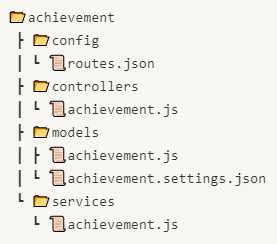
\includegraphics[width=.5\linewidth]{impl/dir_content_type.png}
    \caption{Aufbau eines Inhaltstypen am Beispiel des \textit{Achievement}-Inhaltstypen}
    \label{fig:impl-backend-content-type}
\end{figure}

In der Konfigurationen werden die verschiedenen API Routen des Inhaltstypen
festgelegt. Für jede Route wird die HTTP-Methode, der entsprechende Pfad (z. B.
\textit{/achievements/:id}) und eine Kontroller-Funktion zugewiesen. Bei der
Wahl der HTTP-Methode ist die Funktion der Route zu beachten und sollte der von
\textcite{RFC7231} beschriebenen Semantik folgen. Beispielweise sollte eine
Anfrage, welche lediglich Daten zurückerhalten möchte, die \textit{GET}-Methode
nutzen. Eine Anfrage, welche mir übermittelten Daten einen neuen Eintrag im
System erschafft sollte hingegen die \textit{POST}-Methode nutzen. Alle
voreingestellten Routen sind in \autoref{table:impl-backend-routes} aufgelistet.
Die eingehenden Anfragen werden von der angegebenen Kontroller-Funktion
verarbeitet. \\
Der Kontroller besteht aus Funktionen, welche, wie zuvor beschrieben, ausgeführt
werden, wenn eine für sie hinterlegte Anfrage erhalten wird. In der Anfrage
enthaltene Daten (z. B. abgeschlossenes Abzeichen) werden an die Funktion
übergeben. Innerhalb der Kontroller-Funktion wird die Anfrage verarbeitet und
eine Antwort zurückgesendet. Die Antwort können dabei ein beliebiger
HTTP-Statuscode, binäre Daten oder Daten in JSON-Form sein.
\\
Das Modell bestimmt die Datenstruktur eines Inhaltstypen und nutzt dabei von
Strapi vorgegebene Datentypen (s. \autoref{fig:impl-backend-types}). Jeder
Inhaltstyp setzt sich aus ein oder mehreren Attributen zusammen, welche aus
einem Namen und einem der Datentypen zusammensetzen. Die Attribute können direkt
in der entsprechenden Datei angelegt oder in der Oberfläche von Strapi
festgelegt werden (s. \autoref{fig:impl-backend-content-type-builder}).
\\
Dienste werden genutzt, um duplizierten Code zu vermeiden. Logik, welche an
mehreren Stellen der benötigt wird, kann in einen Dienst geschrieben werden, um
von dort aus in der API benutzt zu werden. Somit fällt der duplizierte Code weg,
was den Code übersichtlicher und leichter anpassbar macht.

\begin{table}[htpb]
    \def\arraystretch{1.25}
    \centering
    \caption{Voreingestellte Routen von Strapi Kollektionen am Beispiel der Abzeichen}
    \label{table:impl-backend-routes}
    \begin{tabular}{lll}
        \uzlhline%
        \uzlemph{Methode} & \uzlemph{Route}              & \uzlemph{Funktion}              \\
        \uzlhline%
        GET               & \textit{/achievements}       & Erhalte alle Abzeichen-Einträge \\
        GET               & \textit{/achievements/:id}   &
        Erhalte Abzeichen-Eintrag mit der angegebenen ID                                   \\
        GET               & \textit{/achievements/count} &
        Erhalte Anzahl der Abzeichen-Einträge                                              \\
        POST              & \textit{/achievements}       &
        Erstellen eines Abzeichen-Eintrags                                                 \\
        DELETE            & \textit{/achievements/:id}   &
        Löschen des Abzeichen-Eintrags mit der angegebenen ID                              \\
        PUT               & \textit{/achievements/:id}   & Verändern des
        Abzeichen-Eintrags mit der angegebenen ID                                          \\
        \uzlhline
    \end{tabular}
\end{table}

\begin{figure}[htpb]
    \centering
    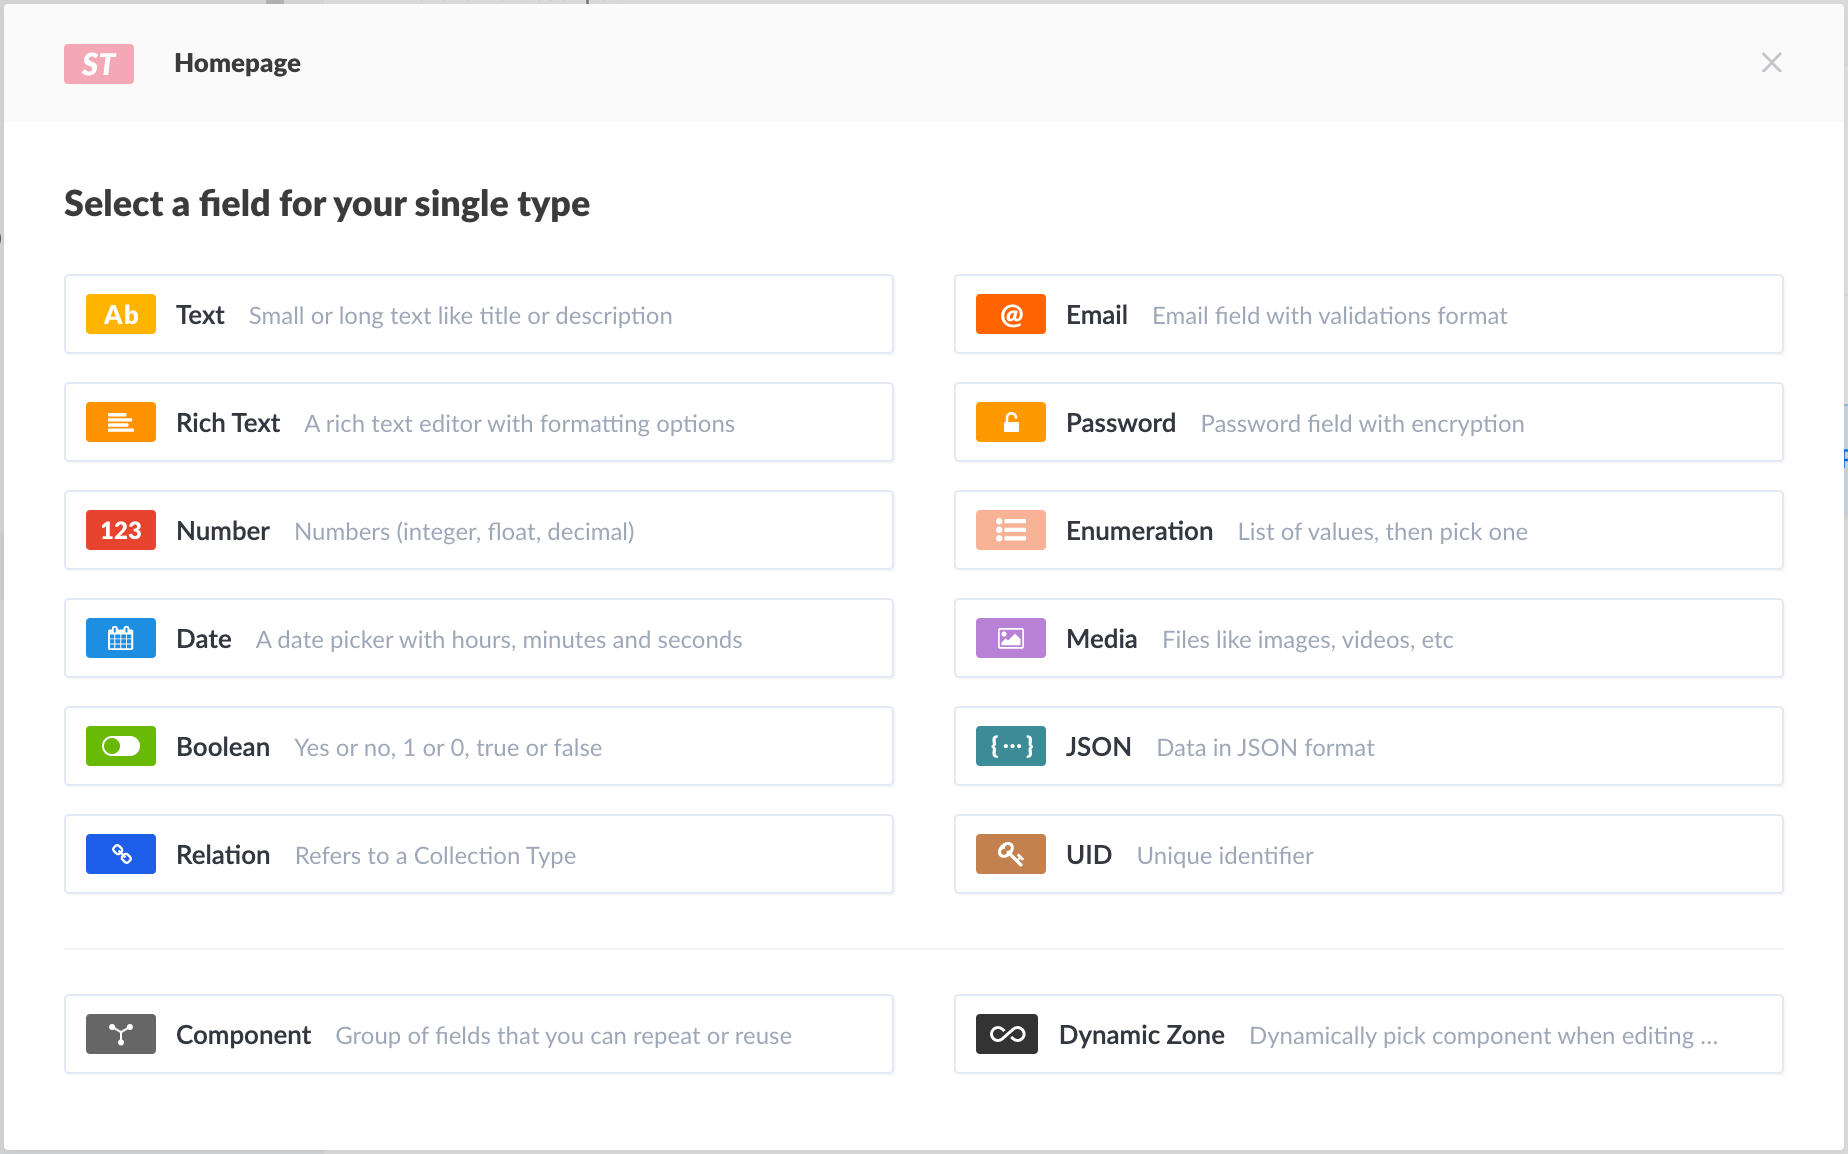
\includegraphics[width=\linewidth]{impl/types.png}
    \caption{Auflistung der verfügbaren Datentypen für Attribute von Inhaltstypen innerhalb Strapis}
    \label{fig:impl-backend-types}
\end{figure}

\begin{figure}[htpb]
    \centering
    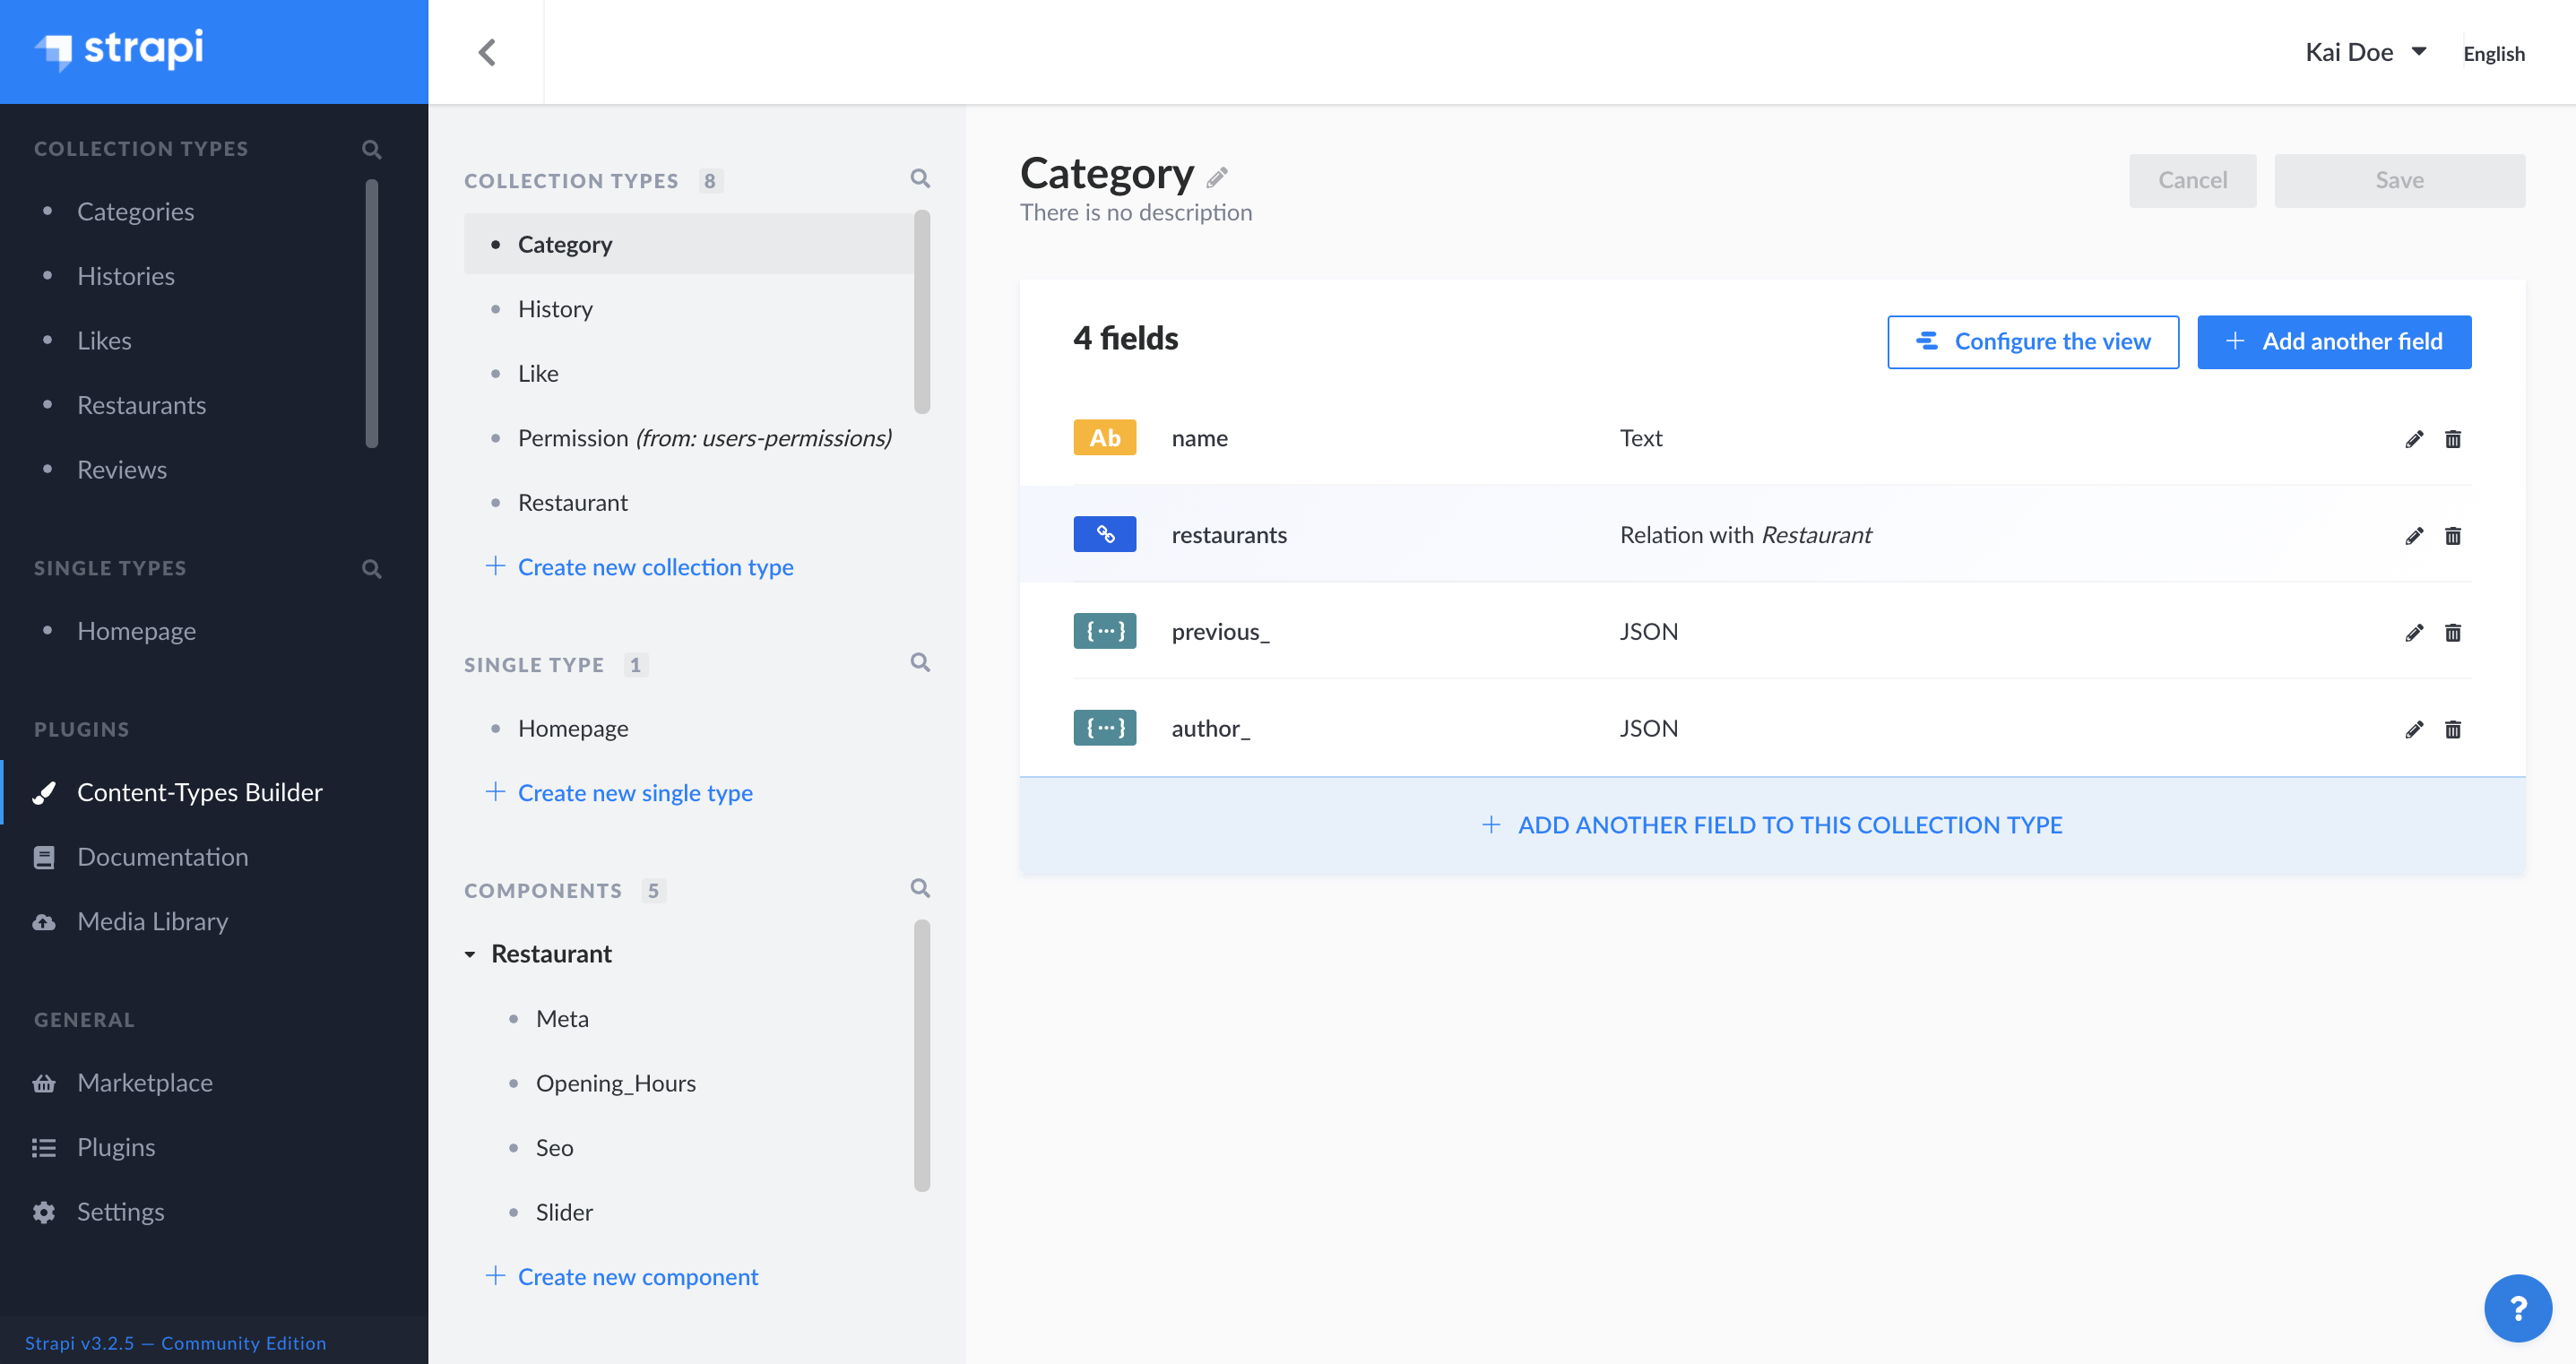
\includegraphics[width=\linewidth]{impl/content-types-builder.png}
    \caption{Oberfläche zum Festlegen der Datenstruktur}
    \label{fig:impl-backend-content-type-builder}
\end{figure}

Das \lstinline[style=code, style=inline]{/config/functions} Verzeichnis des
Projekts enthält Code, welcher zum Start des Systems ausgeführt wird. Die von
der \lstinline[style=code, style=inline]{bootstrap.js} exportierte Funktion
wurde hierbei genutzt, um einen Web-Socket Server zu starten und benötigte
Berechtigungen zu setzen. Auf diese Punkte wird in
\ssecref{ssec:impl-backend-push} genauer eingegangen.

Das \lstinline[style=code, style=inline]{/plugins} Verzeichnis kann genutzt
werden, um Strapi um eigene Module zu erweitern. Möglich ist unter anderem das
Hinzufügen von eigenen Seiten innerhalb der Oberfläche oder die Einbindung einer
eigenen Oberfläche zur Bearbeitung von Attributen. In diesem Projekt sind drei
Plugins zu finden: \textit{groups, dashboard} und \textit{location-picker}. Das
Gruppen-Plugin erfüllt eine Funktion im Backend und wird in
\ssecref{ssec:impl-backend-func} näher erläutert. Das Dash\-board und
Location-Picker-Plugin hingegen werden in \autoref{sec:impl-dashboard}
beschrieben.

Abschließend befinden sich im \lstinline[style=code, style=inline]{/tests}
Verzeichnis Softwaretests, welche genutzt werden, um die korrekte Funktionsweise
der Funktionalitäten, wie in \autoref{sec:concept-func} spezifiziert,
sicherzustellen. Diese sind im Veranstaltungskontext besonders wichtig, da
Fehler während der Veranstaltung im schlimmsten Fall eine komplette
Unterbrechung bedeuten könnten (\anfref{Q30}).

\subsection{Implementierung der Kern-Funktionalitäten} \label{ssec:impl-backend-func}

Nachfolgend wird die Implementierung der Kern-Funktionalitäten des Backends
erläutert, welche aus den Anforderungen aus \autoref{sec:analysis-anf} entnommen
werden. Konkret werden im Folgenden die Implementierung der Stationsbesuche,
Abzeichen und Gruppen erläutert.

Das Besuchen von Stationen erfolgt mithilfe der Übermittlung des Stations-Codes,
welcher aus vier Zeichen, begrenzt auf Zahlen und großen Buchstaben, besteht.
Der Stations-Code ist unabhängig von der ID der Station und kann manuell
festgelegt werden. Dieses Vorgehen ist nötig, da die inkrementellen IDs der
Stations-Kollektion zu einfach zu erraten wären. Zudem können Stations-Codes so
im Nachhinein angepasst werden, sollte z. B. ein Fehler im Druck von QR-Codes
passieren. Eine wichtige Einschränkung bei Stationsbesuchen ist das Verbot von
mehrmaligem Besuchen. Um diese Einschränkung sicherzustellen wurde das Besuchen
von Stationen in einer eigenen \textit{Visit} API realisiert. Die Interaktion
mit der Visit API wird in \autoref{fig:impl-backend-visit-seq} vereinfacht dargestellt.

\begin{figure}[htpb]
    \centering
    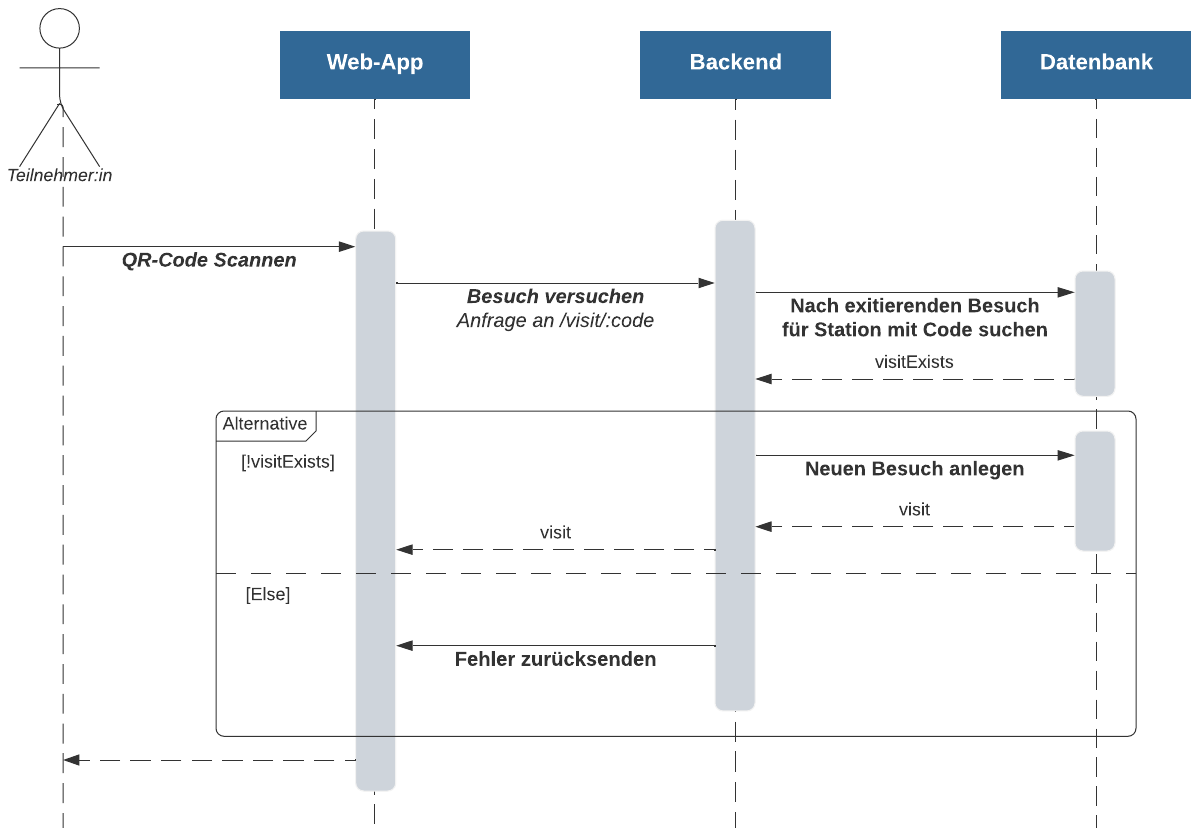
\includegraphics[width=\linewidth]{impl/sequence_visit.png}
    \caption{Interaktion eines Teilnehmenden mit der Visit API}
    \label{fig:impl-backend-visit-seq}
\end{figure}

Um eine Station zu besuchen, wird eine POST Anfrage an \textit{/visit/:code}
abgeschickt, wobei \textit{:code} den Code der Station darstellt. Sollten
Teilnehmende die angegebene Station bereits besucht haben, wird ein
entsprechender Fehlercode zurückgegeben. Andernfalls werden die Daten des
Besuchs, inklusive der Stations-ID, zurückgegeben, um in der Web-App die
Weiterleitung zur entsprechenden Stationsseite zu ermöglichen. Die Datenstruktur
der Stationsbesuche ist in \autoref{fig:impl-backend-visit-data} zu sehen.

\begin{figure}[htpb]
    \centering
    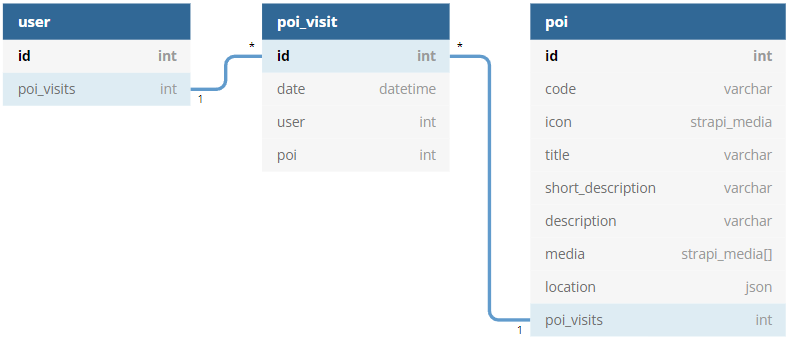
\includegraphics[width=\linewidth]{impl/uml_poi.png}
    \caption{Datenstruktur der Station in Verbindung mit Nutzenden. Intern werden Stationen als \textit{poi} (Point of Interest)
        bezeichnet.}
    \label{fig:impl-backend-visit-data}
\end{figure}

Die Stationsbesuche werden dabei bewusst in einer separaten Tabelle gespeichert,
um die Daten später einfacher zu filtern und das Speichern des Besuch-Zeitpunkts
zu ermöglichen.

Das Abschließen von Abzeichen besitzt, für Bild- und Textabzeichen, einige
Parallelen zum Besuchen von Stationen. Auch hier gilt die Einschränkung, dass
ein bereits eingereichtes Abzeichen nicht erneut eingereicht werden können soll,
solange die Einreichung nicht abgelehnt wurde. Hierfür wurde ebenfalls eine
weitere API hinzugefügt: die \textit{Complete} API. Die Interaktion von
Teilnehmenden mit der Complete API ist in
\autoref{fig:impl-backend-complete-seq} grafisch aufbereitet.

\begin{figure}[ht]
    \centering
    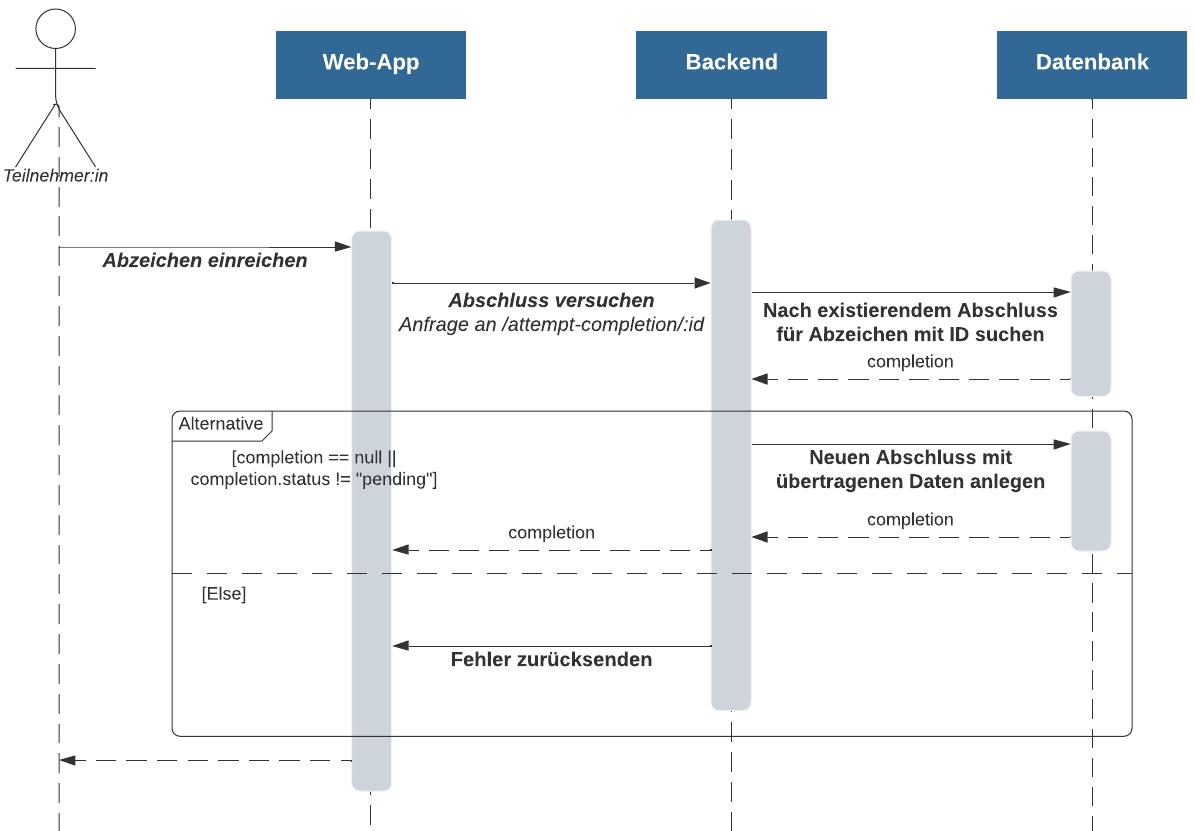
\includegraphics[width=\linewidth]{impl/sequence_completion.png}
    \caption{Interaktion eines Teilnehmenden mit der Complete API}
    \label{fig:impl-backend-complete-seq}
\end{figure}

Um ein Text- oder Bildabzeichen abzuschließen, wird eine POST Anfrage an
\textit{/attempt-completion/:id} abgeschickt, wobei \textit{:id} die ID des
Abzeichens darstellt. Bei vorhandener ausstehender Abgabe wird ein Fehlercode
zurückgegeben. Andernfalls wird die übertragene Einreichung in der Datenbank des
Backends gespeichert. Im Gegensatz zur Visit API wird die Complete API auch von
Veranstaltenden genutzt, um Einreichungen zu bewerten. Über das in
\autoref{sec:impl-dashboard} beschriebene Dashboard können Veranstaltende die
Einreichung akzeptieren oder ablehnen. Daraufhin wird eine Anfrage an
\textit{/complete/:id} bzw. \textit{/dismiss/:id} gesendet, wobei die ID des
Abschlussversuchs übergeben wird (vgl.
\autoref{fig:impl-backend-complete-seq-v}). Wird der Abschlussversuch gefunden
wird der entsprechende Status darin gesetzt. Mögliche Statusangaben sind
„pending“, „denied“ und „accepted“. Der „pending“ Status wird dabei
ausschließlich beim Erstellen des Versuchs verwendet. Diese Logik wird jedoch
nur für Text- oder Bildabzeichen genutzt. Für alle anderen Abzeichen wird die
entsprechende Bedingung im Code überprüft und bei erfüllter Bedingung direkt
ein Eintrag mit „accepted“ für das jeweilige Abzeichen erstellt.

\begin{figure}[htpb]
    \centering
    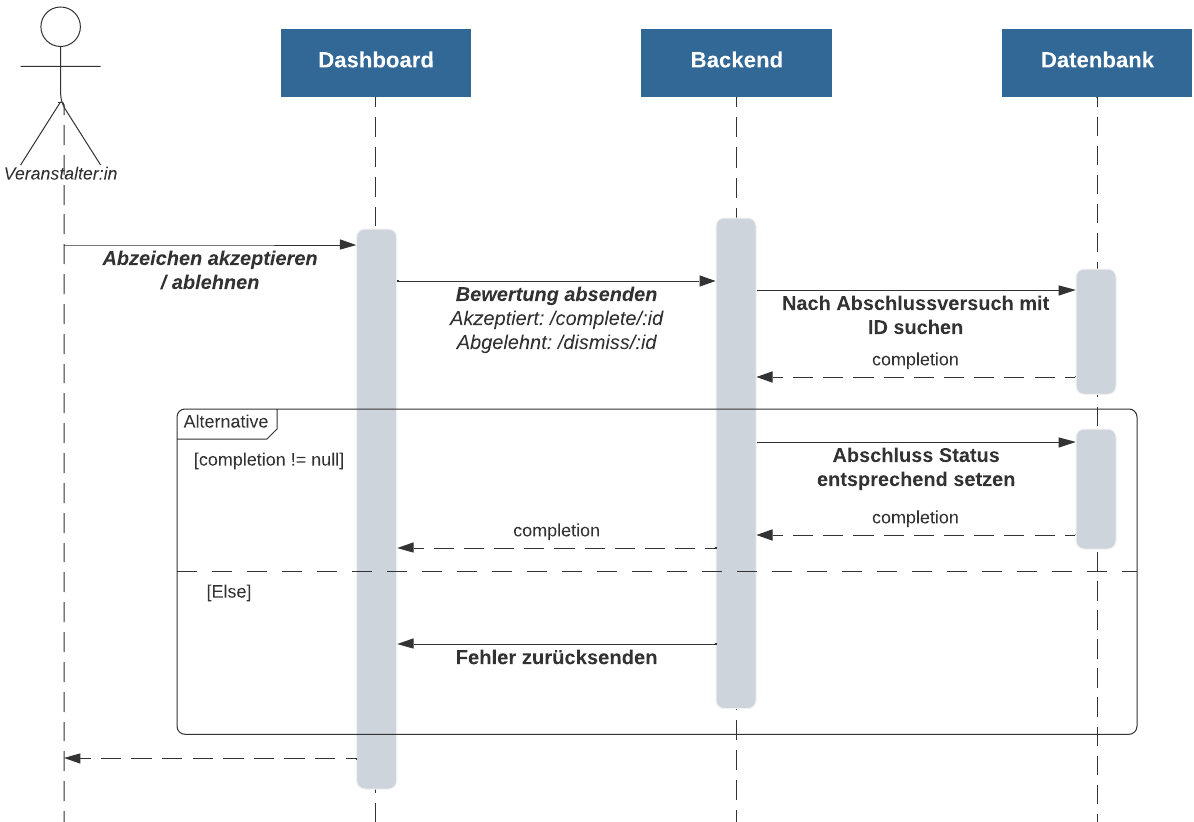
\includegraphics[width=\linewidth]{impl/sequence_completion_v.png}
    \caption{Interaktion eines Veranstaltenden mit der Complete API zum Bewerten einer Einreichung}
    \label{fig:impl-backend-complete-seq-v}
\end{figure}

Ähnlich zur Datenstruktur des Stationsbesuchs werden auch Abzeichen und ihre
dazugehörigen Abschlüsse auf zwei Tabellen aufgeteilt (s. \autoref{fig:impl-backend-completion-data}). Der Grund hierfür ist
ebenfalls die Erfassung der Erstellungs- und Bewertungszeit, sowie die einfache
Durchsuchung.

\begin{figure}[htpb]
    \centering
    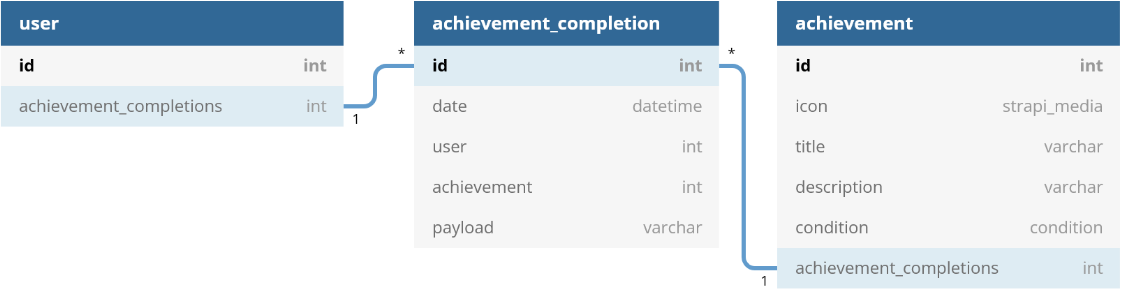
\includegraphics[width=\linewidth]{impl/uml_achievement.png}
    \caption{Datenstruktur der Abzeichen in Verbindung mit Nutzenden}
    \label{fig:impl-backend-completion-data}
\end{figure}

\newpage

Die Gruppen-Funktionalität erweitert Stationsbesuche und Abzeichen, indem
Besuche und Abschlüsse nicht mit Teilnehmenden, sondern analog mit deren Gruppe
verknüpft werden. Sobald ein Gruppenmitglied eine Station oder ein Abzeichen
abschließt, gilt dies somit für alle Mitglieder einer Gruppe. Da die
Gruppen-Funktionalität von Veranstaltenden optional oder ausgeschaltet werden
kann, muss es für Teilnehmende trotzdem möglich sein, diese Aktionen einzeln
auszuführen. Somit ergibt sich die in \autoref{fig:impl-backend-groups-data}
gezeigte Datenstruktur.

\begin{figure}[htpb]
    \centering
    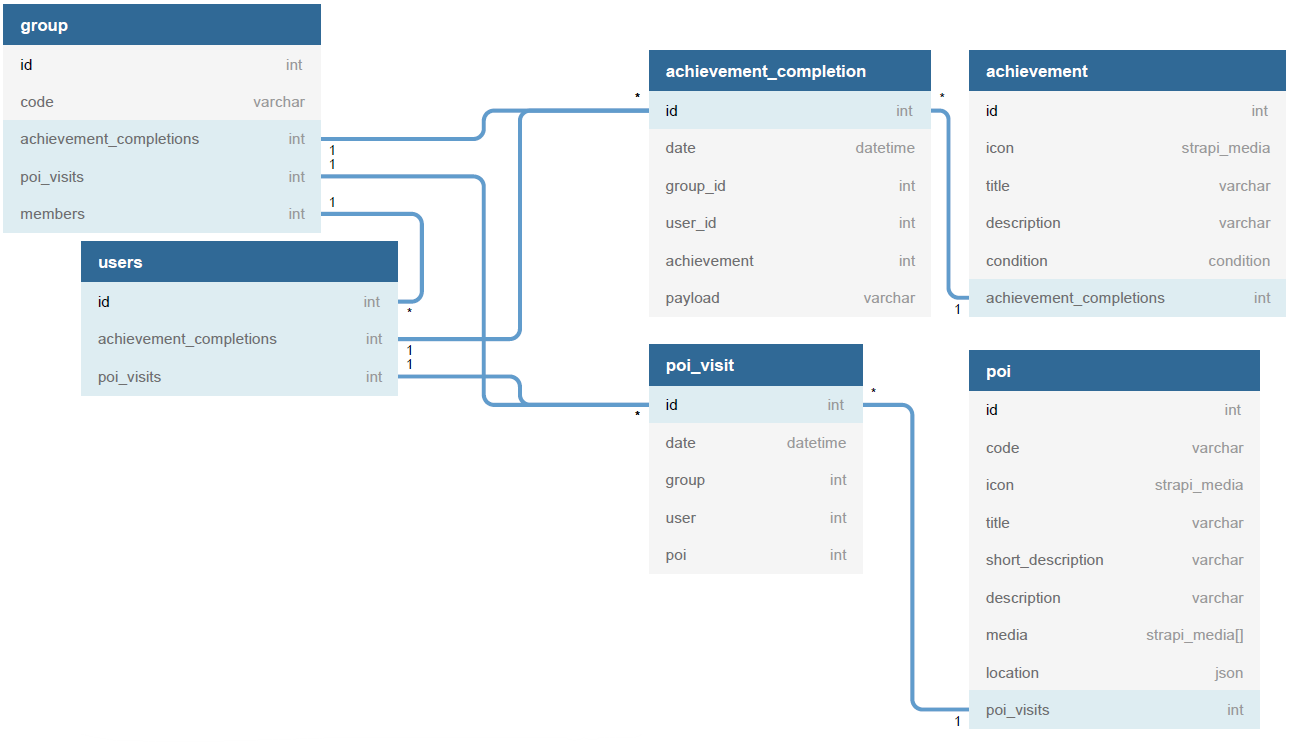
\includegraphics[width=\linewidth]{impl/uml_poi_achievement_group.png}
    \caption{Datenstruktur der Abzeichen und Stationen im Zusammenhang mit Gruppen}
    \label{fig:impl-backend-groups-data}
\end{figure}

Bevor Teilnehmende gemeinsam in einer Gruppe agieren können, müssen sie diese
erstellen oder ihr beitreten. Dies geschieht über eine POST Anfrage an die
\textit{/groups/create} oder \textit{/groups/join} Route. Der
\textit{/groups/create} Route muss zusätzlich der Name der zu erstellenden
Gruppe übermittelt werden, während die \textit{/groups/join} Route den
Gruppen-Code der beitretenden Gruppe benötigt. Abschließend kann die Gruppe auch
wieder verlassen werden, indem eine POST Anfrage an die \textit{/groups/leave}
Route geschickt wird.
\\
Sobald Teilnehmende Mitglied einer Gruppe sind, wird bei Stationsbesuchen und
Abzeichen Einreichungen oder Abschlüssen die Gruppe, statt der Teilnehmenden,
hinterlegt. Gleichzeitig wird beim Auslesen der Besuche und Abschlüsse nicht
mehr nach der Nutzer-ID, sondern der Gruppen-ID gefiltert. Alle
Gruppenmitglieder erhalten somit die neu erstelle Aktion. Eine Einschränkung
dieses Systems ist der temporäre Verlust von Daten bei Beitreten oder Verlassen
einer Gruppe, da jeweils nur Gruppen- bzw. Einzeldaten berücksichtigt werden.
Sobald Teilnehmende ihre Gruppe verlassen, werden wieder Einzeleinträge
angezeigt, da die Gruppeneinträge nicht mehr mit den Teilnehmenden
assoziiert sind. Dies gilt analog auch für das Beitreten einer Gruppe.

\subsection{Implementierung der Push-Benachrichtigungen} \label{ssec:impl-backend-push}
\label{ssec:impl-backend-push}

Gemäß \textit{Ft-V-5} (s. \ssecref{ssec:func-new}) sollen Teilnehmende von
Veranstaltenden jederzeit benachrichtigt werden können. Im Web-Kontext kann dies
über die Web-Push API erfolgen, welche es ermöglicht, auch außerhalb der Nutzung
der Web-App Benachrichtigungen zu erhalten. Jedoch wird die Web-Push API nicht
von Safari auf iOS unterstützt \cite{MDN2021}, weshalb eine Rückfalllösung
gebraucht wird. Unter Beachtung dieser Beschränkungen wurde ein drei-stufiges
Verfahren entwickelt, welches sich aus der Push API und einem Web-Socket Server
zusammensetzt. Im Folgenden werden diese beiden Technologien näher vorgestellt
und ihre Aufgabe und Interaktion im System präsentiert.

Der Web-Push Standard ermöglicht das Versenden und Empfangen von
Push-Benach\-richti\-gungen im Web-Kontext. Ein Endgerät, wie z. B. ein Smartphone
mit Browser, kann durch die Push API einen Push-Dienst abonnieren. Durch das
Abonnieren erhält das Endgerät eine eindeutige URL, welche von einem Server, wie
z. B. dem Backend, genutzt werden kann, um jederzeit Nachrichten an das Endgerät
zu senden. Ein besonderer Vorteil der Web-Push Standards ist das Versenden von
Nachrichten außerhalb der Browsernutzung. Sollten Teilnehmende die Web-App zum
Zeitpunkt des Versendens nicht ausführen, so wird die Nachricht trotzdem
empfangen. Die Funktionsweise der URL birgt jedoch ein Sicherheitsrisiko, da
jeder mit dieser URL beliebige Nachrichten an das entsprechende Endgerät senden
kann. Um diese Sicherheitslücke zu schließen, muss jedes Abonnement
verschlüsselt werden. Dies geschieht mit VAPID-Schlüsseln \cite{VAPID}, wodurch
auf dem Endgerät sichergestellt werden kann, das die Nachricht vom richtigen
Server stammt.

Web-Sockets hingegen sind für die Echtzeit-Kommunikation zwischen Endgerät und
Server gedacht. Sie ermöglichen das Senden und Empfangen von Nachrichten in
beide Richtungen. Somit kann das Endgerät, im Gegensatz zum Web-Push Standard,
auch Nachrichten an den Server schicken. Hierzu wird eine dauerhafte Verbindung
mit dem Server aufgebaut, welche jedoch mit dem Schließen der Web-App abbricht.
Im Vergleich zum Web-Push Standard eigenen sich Nachrichten über Web-Sockets
somit nur während der Nutzung der App. Jedoch werden für Web-Sockets keine
weiteren Verschlüsselungsmethoden, neben der Nutzung von HTTPS, benötigt. Zudem
vereinfachen JavaScript-Bibliotheken wie Socket.IO\footnote{https://socket.io/},
welche in dieser Arbeit verwendet wurde, die Nutzung von Web-Sockets und
verwenden intern weitere Methoden um eine stabile Verbindung über eine
breite Auswahl an Geräten zu garantieren \cite{SocketIO2022}.


Basierend auf den Fähigkeiten der beiden vorgestellten Technologien wird ein
drei-stufiges Verfahren zur Benachrichtigung entwickelt, welches in
\autoref{fig:impl-backend-push} präsentiert wird. Wenn Veranstaltende eine
Nachricht versenden, wird zunächst das Versenden mit Web-Push versucht. Sollte
dies fehlschlagen, wird die Nachricht stattdessen über eine Web-Socket
Verbindung versendet. Falls auch dies fehlschlägt, wird die Nachricht im
Nutzerprofil gespeichert. Sobald Teilnehmende sich wieder mit dem Server
verbinden, wird dieser Vorgang erneut versucht. Allerdings wird die Nachricht in
diesem Fall verworfen, sollte die Nachricht weder per Web-Push noch Web-Sockets
versendet werden können (s. \autoref{fig:impl-backend-push-connect}).

\begin{figure}[htpb]
    \centering
    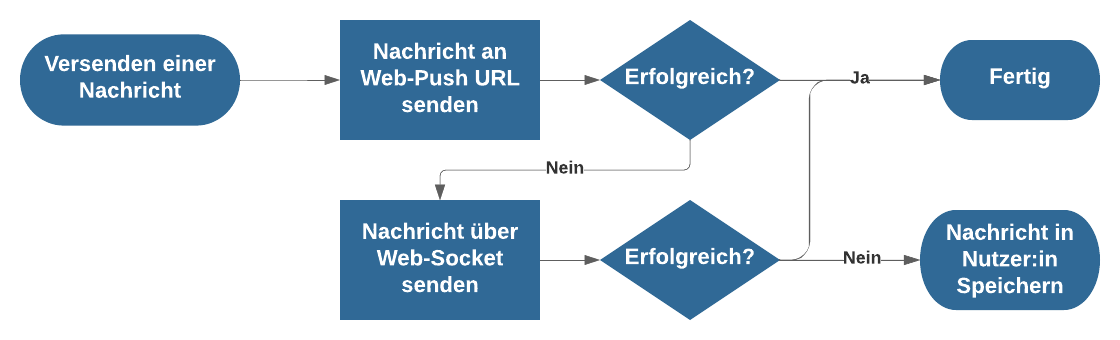
\includegraphics[width=\linewidth]{impl/flow_push.png}
    \caption{Verfahren zum Versenden von Benachrichtigungen an Teilnehmende}
    \label{fig:impl-backend-push}
\end{figure}

\begin{figure}[htpb]
    \centering
    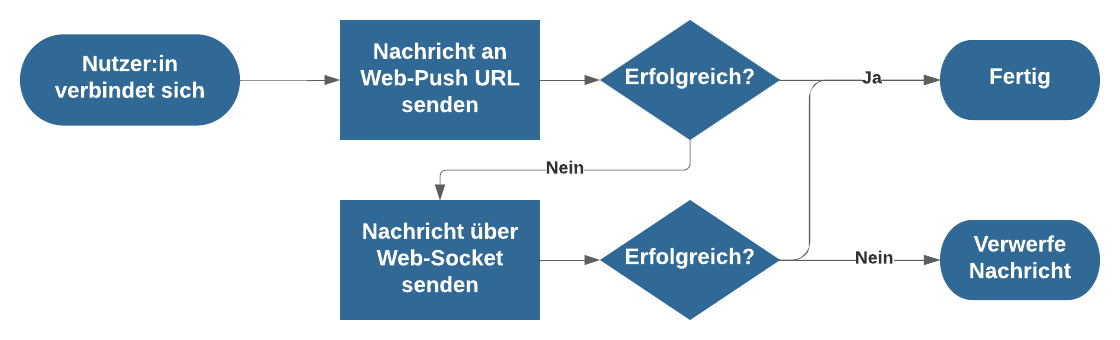
\includegraphics[width=\linewidth]{impl/flow_push_connect.png}
    \caption{Verfahren bei ausstehenden Benachrichtigungen}
    \label{fig:impl-backend-push-connect}
\end{figure}

\subsection{Implementierung der Feedback-Funktionalität}

Die Feedback-Funktionalität baut auf der Implementierung der
Push-Benachrichtigungen auf. Sobald Veranstaltende eine neue Feedback-Anfrage
verschicken, wird diese an alle Teilnehmende über das in
\ssecref{ssec:impl-backend-push} beschriebene Verfahren gesendet. Dabei wird
jede Feedback-Anfrage mit einer eindeutigen ID versehen, um die Antworten später
noch zur jeweiligen Anfrage zuordnen zu können. Die Datenstruktur des
Feedback-Systems wird in \autoref{fig:impl-backend-feedback-data} dargestellt.
Jede verschickte Feedback-Anfrage ist hierbei ein Eintrag in der
\textit{feedback} Tabelle, während die Antworten der Teilnehmenden als Einträge
in der \textit{feedback-response} Tabelle gespeichert werden. Hierzu wird die
Antwort als POST Anfrage an \textit{/feedback/respond} gesendet.

\begin{figure}[htpb]
    \centering
    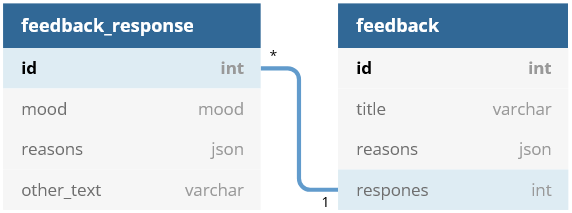
\includegraphics[width=0.6\linewidth]{impl/uml_feedback.png}
    \caption{Datenstruktur des Feedback-Systems}
    \label{fig:impl-backend-feedback-data}
\end{figure}

%\subsection{Softwarequalität}

% - Aussagekräftige Fehlermeldungen ->
% - Softwaretests

\section{Implementierung des Frontend}

\subsection{Struktur mit Vue CLI}

Zur Erstellung und Verwaltung des Projekts wurde das \textit{Vue CLI} genutzt.
Vue CLI ist ein Kommandozeilenprogramm, welches die komplizierte Einrichtung und
Verwaltung von Vue Projekten stark vereinfacht. Das Erstellen eines Projekts
erfolgt nach Installation des Vue CLI durch den Befehl \lstinline[style=code,
    language=bash, style=inline]{vue create <projekt-name>}.

\subsection{Komponentenstruktur}

\subsection{API-Kommunikation}

\subsection{Implementierung der interaktiven Karte}

\subsection{Natives App-Erlebnis}
% Enkodierung des UI-Zustandes in der URL

\subsection{Persistente Nutzerdatenspeicherung}

%!%%%%%%%%%%!%
%! Frontend !%
%!%%%%%%%%%%!%

% inclusive Design
%   - Mehrsprachig
%   - A11y (Aria, W3C Empfehlungen)

% Auf "Refactoring UI"-Standards geachtet

% Tailwindcss Design-System verwendet

% Vue 3
%   - vue-cli
%   - SFC
%   - MVC
%   - Style Guide / Best Practices
%       - script setup (recommended
%         https://v3.vuejs.org/api/sfc-script-setup.html)
%   - Composition API

% Typescript

% Genutzte Libraries:
%   - Axios
%   - MapboxGlJS
%   - marked (Markdown) JSDOMPurify
%   - Iconify
%   - Swiper
%   - Socket.IO

% Gliederung:
%   - Controller
%   - Service
%   - Repository

% Kamera Eigen-Implementierung

% Mapbox Eigen-Implementierung

% Modal Eigen-Implementierung

% Service Worker - Push-Benachrichtigungen

% Optimierungen:
%   - Route Splitting
%   - PWA bzw. Service Worker

\section{Implementierung des Dashboard} \label{sec:impl-dashboard}

\subsection{Aufbau eines Strapi Plugins}

\subsection{Implementierung der Statistiken}

\subsection{Implementierung des Location-Picker Plugins}


\section{Nutzung des Systems}

\subsection{Installation}

\subsection{Ausführung mit Docker}